\documentclass[11pt,a4paper]{article}
\usepackage{fullpage}
\usepackage{graphicx}

\begin{document}

\section*{Theory}
Let us consider the following simplified EMI model 
\begin{eqnarray}
\nabla\cdot(\sigma_i) u_i &=& 0, \mbox{ in } \Omega_i \\
\nabla\cdot(\sigma_e) u_e &=& 0, \mbox{ in } \Omega_e \\
\sigma \nabla u_i \cdot n  -v &=& f \mbox{ on } \Gamma    
\end{eqnarray}
where 
$\Omega_i$ is the intra-cellular domain,  $\Omega_e$ 
is the extra-cellular domain,  and $\Gamma$ is 
the cell membrane. The unknowns $u_i$ and $u_e$ are
intra- and extracellular potientials whereas
$v$ is the transmembrane potential.  
We have interface conditions
\begin{eqnarray}
u_i - u_e &=& v  \\
\sigma_i \nabla u_i \cdot n_i &=& -\sigma_e \nabla u_e \cdot n_e 
\end{eqnarray}
When EMI is considered in cardiac modelling the \emph{interior} domain is
a union of a number of heart cells and $\Gamma$ represents not only the
interfaces between cells and the exterior but the cell-cell interfaces as well,
see Figure \ref{fig:iface_types}. The source terms $f$ on the two interface types
are typically different. Here we shall assume only on interface type.

\begin{figure}
      \begin{center}
     \includegraphics[scale=0.5]{./multi_branches23.mps}
   \end{center}
   \caption{Interface types in the EMI problem. (blue) cell-cell interfaces,
     (red) cell-exterior inerfaces.}
   \label{fig:iface_types}
\end{figure}

The mixed formulation is obtained
by introducing the fluxes $s_i = \sigma_i \nabla u_i$ 
and $s_e = \sigma_e \nabla u_e$. Noting that the flux has continuour normal
component, we may write the above equations 
in weak form as: Find 
$s \in H(\mbox{div}, \Omega)$   
$u \in L^2(\Omega)$   
$v \in H^{1/2}(\Gamma)$  such that 
\begin{eqnarray}
(\sigma^{-1} s, k)_{\Omega} + (u, \nabla \cdot k)_{\Omega} - (v,   n \cdot k)_\Gamma &=& 0 \\    
(\nabla \cdot s, l)_{\Omega} &=& 0 \\ 
(s\cdot n, m)_{\Gamma} - (v, m)_{\Gamma} &=& 0 \\ 
\end{eqnarray}
for
$k \in H(\mbox{div}, \Omega)$   
$l \in L^2(\Omega)$   
$m \in H^{1/2}(\Gamma)$ 
We remark here that the variations
between $\sigma_i$ and $\sigma_e$ are
small, typically order of 10. 

Formally, we may write the system as 
\[
\left(
\begin{array}{ccc}
\sigma^{-1} & (\nabla\cdot)' & T_n' \\
\nabla \cdot & 0 & 0 \\ 
T_n & 0 & -I  
\end{array}
\right)
\left(
\begin{array}{c}
s \\ u \\ v  
\end{array}
\right)
= 
\left(
\begin{array}{c}
f \\ g \\ h  
\end{array}
\right)
\]
and to discretize the problem we would use
Raviart-Thomas elements combined with corresponding discontinuous 
Galerkin for $s$ and $u$. Further, $v$ is only defined on $\Gamma$
and is similarly discretized by discontinuous Galerkin elements
of the same order as $u$. 

In the FEniCS implementation we note that finite elements
on sub-manifolds is still not fully supported, at least not
in parallel. Therefore the space for $v$ shall be setup on \emph{all}
the facets in $\Omega$ and not just on $\Gamma$. As such, we modify the
above system to obtain 
\[
\left(
\begin{array}{ccc}
\sigma^{-1} & (\nabla\cdot)' & T_n' \\
\nabla \cdot & 0 & 0 \\ 
T_n & 0 & -I_f  
\end{array}
\right)
\left(
\begin{array}{c}
s \\ u \\ v  
\end{array}
\right)
= 
\left(
\begin{array}{c}
f \\ g \\ h  
\end{array}
\right)
\]
Here, let $E$ be the set of faces in $\Omega$ (both 
in the interior and at the boundary), then   
\[
I_m (v,m) = \sum_{e \in E}\int_e v m \, \mbox{dS}  
\]
We remark that $I_m$ is a diagonal matrix. 

The question is then: Does BDDC work on this saddle point problem which
is somewhat similar to a standard mixed Darcy problem and is it scalable?

\section*{Practice}

Gmsh version with CAD support (version 3.0.7 and higher) is used to create
the geometry. Since using Gmsh for generation and subsequent meshing of the 
geometry with order 1000 cylinders is not feasible the mesh is created in two 
steps as follows. First we generate a mesh (referred to later as \emph{tile}) 
for one cylinder such that the facets in $x$ and $y$ directions are meshed periodically
\[
\texttt{gmsh -3 -clscale 0.25 tile\textunderscore 1\textunderscore narrow.geo}
\]
With the command below one gets a mesh with element size approximately 3$\mu m$.
\begin{center}
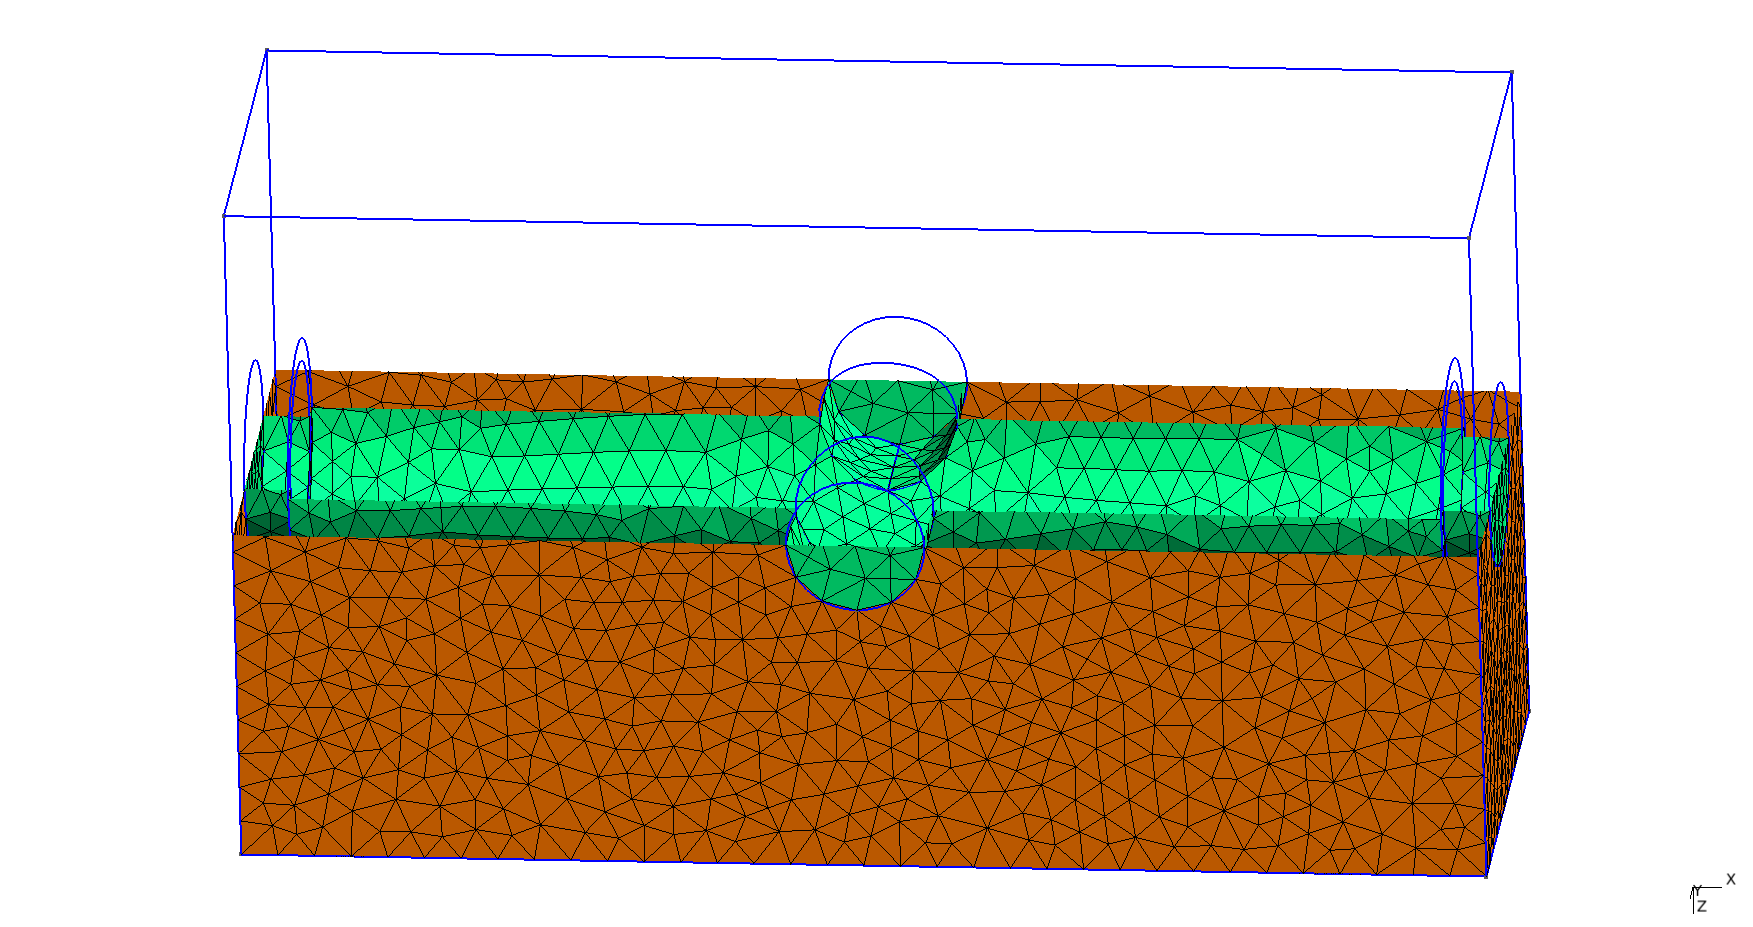
\includegraphics[width=\textwidth]{tile_1.png}
\end{center}
To proceed the mesh is stored in HDF5 format as
\[
\texttt{python msh\textunderscore convert.py tile\textunderscore 1\textunderscore narrow.h5}
\]
Next with glue together the \emph{tiles} together in the periodic directions to 
get the full mesh:
\[
\texttt{python tiling.py tile\textunderscore 1\textunderscore narrow.msh -n 128 -m 128},
\]
where $n, m$ specify the number of tiles in $x$ and $y$ directions. This command 
generated the mesh in approx 500 seconds (most of which was spent generating markers for the 
cell interiors and interfaces) using about 30GB RAM. The mesh takes about 17GB of disk space.
A piece\footnote{I cannot render data from all 32 CPUs at once} of this mesh is shown below 
using some of the cell surfaces (coloring by CPU rank) 
\begin{center}
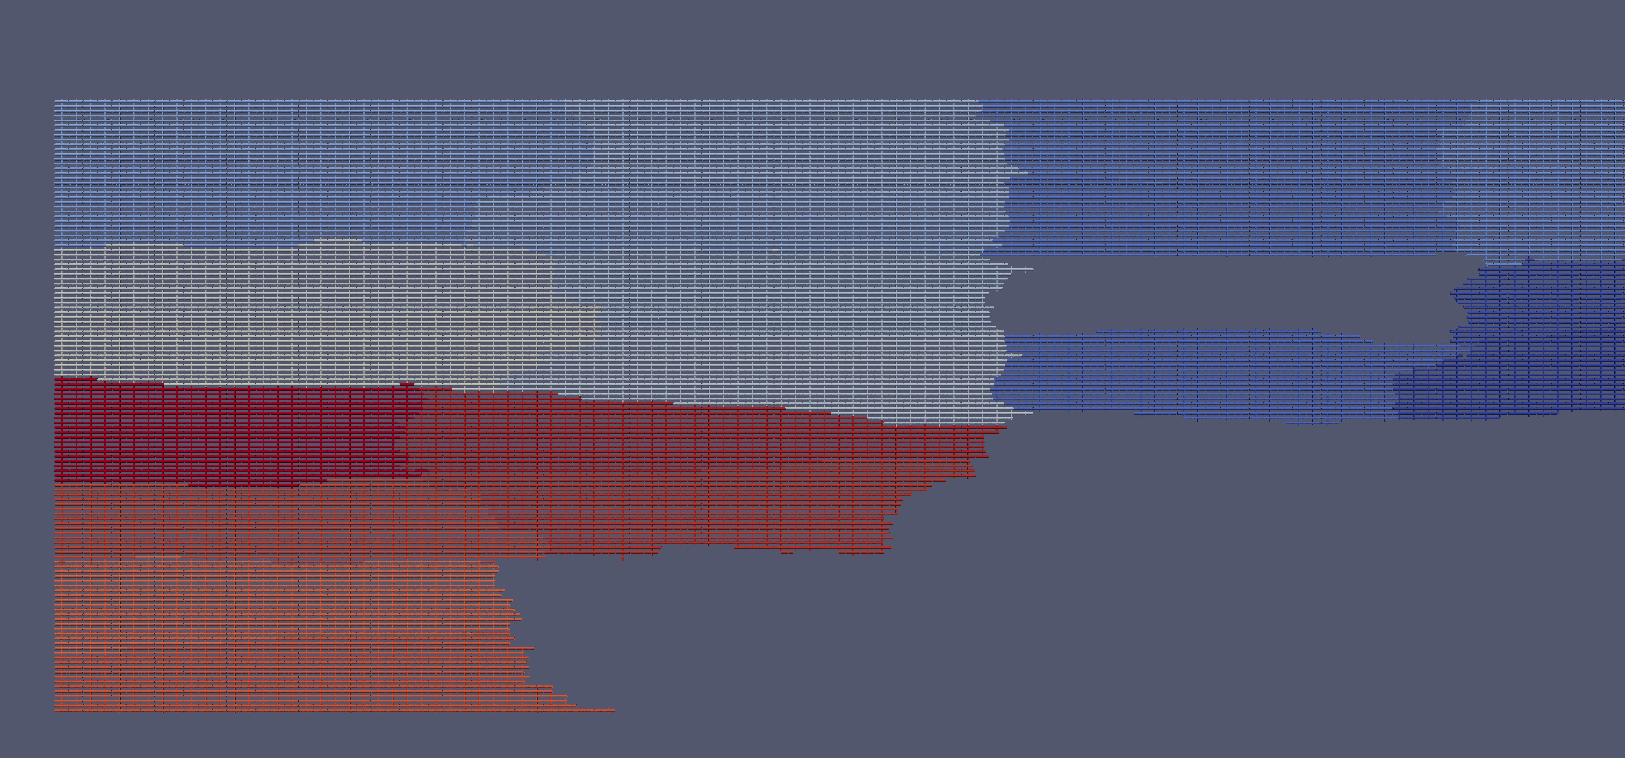
\includegraphics[width=\textwidth]{piece.png}
\end{center}

We remark that we observed factor 4 increase in the execution time/RAM/storage upon doubling 
the $n$ and $m$ counts. 

The computational domain generated above is such that the cells have interfaces which are on 
the boundary of the domain. We currently asume that all the boundary surfaces (including the cells' 
ones) have zero potential. The script for assembling the EMI system with the generated gemetry is
in \texttt{emi\textunderscore system.py}.

% Of the parameters in the script \texttt{cell\textunderscore grid.geo}
% the interesting ones are \emph{nx}, \emph{ny} which control the number of cells
% and thus the length of the interface, see
% \[
% \texttt{gmsh -setnumber nx 2 -setnumber ny 2 cell\textunderscore grid.geo}
% \]
% For mesh generation run
% \[
% \texttt{gmsh -3 -setnumber nx 2 -setnumber ny 2 -clscale 0.5 cell\textunderscore grid.geo}
% \]
% where the number $0.5$ passed to \emph{clscale} instructs to half the characteristic
% mesh sizes set in the script (\emph{size}\textunderscore\emph{box},
% \emph{size}\textunderscore\emph{cell}). The number thus controls resolution
% of the mesh. Two dimensional geometries are generated similarly using
% \[
% \texttt{gmsh -setnumber nx 2 -setnumber ny 2 cell\textunderscore grid\textunderscore 2d.geo}
% \]
% for inspecting and 
% \[
% \texttt{gmsh -2 -setnumber nx 2 -setnumber ny 2 -clscale 1.0 cell\textunderscore grid\textunderscore 2d.geo}
% \]
% for generation of the mesh.

% When Gmsh is done, I convert the \emph{msh} file to HDF5 file format
% using the


\end{document}

